\documentclass[a4paper, 9pt]{article}
\usepackage{../styles}
\title{Lab 4 --- Classification schemes of language and music}
\author{Evolution of Language and Music}
\begin{document}

\maketitle

\begin{goals}
The goals of today's computer lab are to learn about features of
language and music used in comparative research, and about variation
across languages and musics. By studying some specific examples, you
will see that both languages and musical traditions are transmitted
culturally, and are subject to a process of cultural evolution. Finally,
you will see how existing variation in languages and musics can be
harnassed to reconstruct the cultural evolutionary history, using very
similar methods as we saw for phylogenetic tree reconstruction of
species and genomes.
\end{goals}

\section{Introduction}\label{introduction}

The principles of evolution can in theory be applied to any system where
the basic ingredients of evolution---variation, inheritance and
selection---are present. The cultural transmission of languages and
music is an example of such a system. It is possible to study the
\emph{cultural} evolution of language and music. But how do we start
start to disentangle phylogenetic relationships between cultural
phenomona like language and music? One possibility is to, just as we
would for biological species, apply the comparative method.

Before we can start comparing, we need some systematic way of expressing
how cultural phenomena how they are different and to what extent. For
this purpose, \emph{classification schemes} are commonly used.
Classification schemes can be used to \emph{encode} a particular product
of cultural evolution (such as musical traditions and languages) into a
set of \emph{features}. An example of a feature is whether a musical
tradition involves drumming. Once we have an encoded representation of a
language or musical tradition, we can quantify similarity \emph{between}
languages and musical traditions. This allows us to study them with
comparative methods such as phylogenetic analysis (as we've done in
previous labs).

Encoding a language or music into features sometimes requires strong
expertise (for example, speaking a language as well as having in depth
knowledge of its structure is required for deciding on whether certain
linguistic features are present in a language). In this lab we will get
a taste for what is involved with encoding. Furthermore, the way a
product of cultural evolution is coded into features is not always
unambiguous.

In this lab we'll look some language and music features in detail and
study their uses.

\section{Part 1: Music}\label{part-1-music}

Although music is found in every human culture on this planet, the
diversity in style and cultural role of music is enormous. Whether any
aspect of music is universal to all these cultures is the topic of
heated debate.

Savage et al. derive 32 \emph{binary} features (features that can have
just two possible values: \textbf{1} for present and
\textbf{0} for absent) from existing classification schemes to
empirically test the validity of many of the candidate universals
proposed by \cite{Brown2013}. Using this classification scheme, Savage
et al. \emph{encode} each recording as a vector indicating the presence
or absence of each of the 32 features. These binary features were used
to encode 304 recordings from the \emph{Garland Encyclopedia of World
Music} into feature vectors. The 304 recordings originate from a wide
variety of regions, as can be seen in figure \ref{fig:garland}.

\begin{exercise}
\askstar Which of the following features of an organism are binary?
\begin{itemize}
\item The color of the organism's hair.
\item The organism's average walking speed.
\item Whether the organism is bipedal.
\item The amount of wings on the organism.
\item The ability to remain under water for longer than 5 minutes.
\end{itemize}
\end{exercise}

Note that while classification schemes for language often apply to a
language as a whole, as spoken by people from a certain geographical
region, Savage et al. apply a classification scheme to individual
recordings.

\begin{exercise}
\askstar When applying classification schemes to music, what would be a reason to use individual recordings, instead of, say, using music from a certain geographical region?
\end{exercise}

\begin{figure}
\center
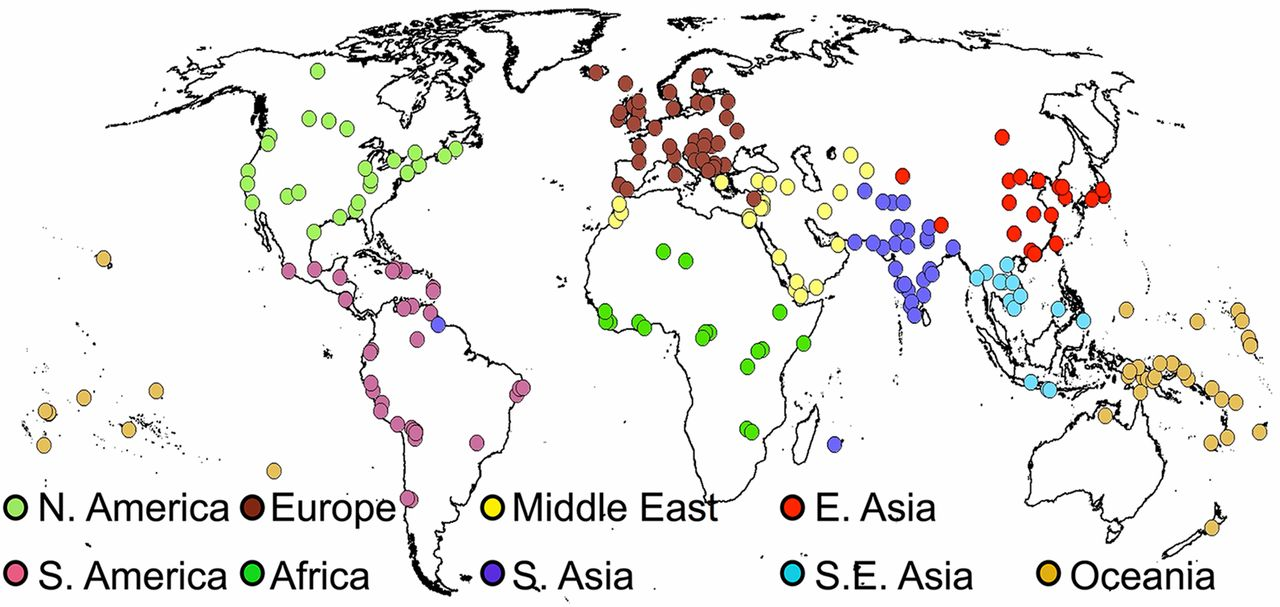
\includegraphics[width=0.8\linewidth]{img/geo-distribution-garland}
\caption{Origins of the 304 recordings in the \textit{Garland Encyclopedia of World Music}. Figure from \cite{Savage2015}}
\label{fig:garland}
\end{figure}

The University of Amsterdam has access to all recordings that were used
in the study. When connected to the university network (through a lab
computer or eduroam), you can access them here:
\url{http://search.alexanderstreet.com/glnd}.

\begin{exercise}
\action Go to the website given above and listen to some recordings from at least three different continents. 
\end{exercise}

We'll look at three of the features used by Savage et al. in detail:
(the presence or absence of) isochronous beat, metrical hierarchy, and
discrete pitches. You've heard about the concepts these features encode
in class. In order to get a feeling for what they mean, we'll step into
an ethnomusicologist's shoes and identify some of these features in
recordings of various styles of music from all over the world.

\subsection{Isochrony}\label{isochrony}

The feature \emph{isochronous beat} is present when time is divided
clearly into equal units. In general, music with an isochronous beat is
music that you can imagine clapping or tapping along with.

To get a feel for what isochrony means, we'll first listen to an example
that clearly has an isochronous beat.

\begin{exercise}
\action Listen to track 7 (Anlo-Ewe kinka songs ) from the Vol. 1: Africa CD.
\end{exercise}

An example that clearly lacks an isochronous beat is the following:

\begin{exercise}
\action Listen to track 9 (Thai Dam khap  singing) from the Vol. 5: Southeast Asia CD.
\end{exercise}

Sometimes the presence or absence of an isochronous beat is clear and
unambiguous, like in the previous two examples. However, things are not
always this clear-cut.

\begin{exercise}
\action Listen to track 2 (Coiled Chalk Circle) from the Vol. 3: North America CD.
\action Listen to track 7 (Personal song) from the Vol. 3: North America CD.
\end{exercise}

The first of these recordings was classified by Savage et al. as
containing an isochronous beat, whereas the second was classified as
lacking an isochronous beat.

\begin{exercise}
\askstar Draw a little diagram to illustrate the difference between isochronous and non-isochronous music. 
\end{exercise}

\subsection{Metrical hierarchy}\label{metrical-hierarchy}

Music with an isochronous beat contains a pulse you can tap or clap
along with. When slower or faster pulses are present that fit
hierarchically in the pulse that you clap or tap along with we speak of
a \emph{metrical hierarchy}. For example, it could be that each pulse is
subdivided in three (isochronous) faster pulses, or it might be that
every three pulses sounds stronger such as in a Walz, where you
generally count pulses as one-two-three one-two-three etc. Most Western
music that has an isochronous beat also has metrical hierarchy.

The feature \emph{metrical hierarchy} is subordinate to isochronous
beat. If an isochronous beat is not present, metrical hierarchy is not
applicable.

\begin{exercise}
\action Listen to track 21 from the Vol. 8: Europe CD.
\end{exercise}

This song has a clear metrical hierarchy: you can group the isochronous
pulses in groups of four, where the first one sounds somehow more strong
(try counting along by counting one-two-three-four one-two-three-four,
etc. along with the isochronous pulse).

\begin{exercise}
\action Listen to track 17 (Canto a lo peuta) from the Vol. 2: South America CD.
\end{exercise}

Although there clearly is an isochronous beat, this song lacks metrical
structure; there seems to be no coherent shorter or faster pulse that
you can count or clap along with.

\begin{exercise}
\askstar Draw a little diagram to illustrate the concept of (a) metrical hierarchy. 
\end{exercise}

\subsection{Discrete pitches}\label{discrete-pitches}

When the sung pitches are clearly separated from each other small steps,
we speak of \emph{discrete pitches}. Most recordings in the dataset
contain discrete pitches. However this feature is coded as absent when
the lyrics are whispered (e.g.~track 3 from vol.~1) or spoken, or when a
recording contains purely percussion (e.g.~track 17 from vol.~5).


\subsection{Classification}\label{classification}

Finally, we will try and classify some recordings ourselves.

\begin{exercise}
\action Copy the table below, listen to the listed recordings and try to code them in terms of the three listed features that we discussed above. 
\end{exercise}

\[
\begin{tabular}{lllll}
\textbf{Volume} & \textbf{Track} & Isochronous beat & Metrical hierarchy & Discrete pitches \\
\hline
3 (North America) & 7 &  & & \\
6 (Middle East) & 19 &  & & \\
6 (Middle East) & 27 &  & & \\
8 (Europe) & 9 &  & & \\
9 (Oceania) & 52 &  &  &  \\

\end{tabular}
\]

\section{Part 2: Language}\label{part-2-language}

\subsection{Cognates}\label{cognates}

One way of establishing relatedness of languages is to quantify how many
words they have that have a common (etymological) origin. Such words are
called cognates. To get a feeling for what cognates are, we will start
by identifying cognates in two sentences we can easily find translations
of in many languages: two sentences from the declaration of human
rights\footnote{for other languages, or more sentences from the same language, you can check http://unicode.org/udhr/assemblies/full\_all.txt}
and the favourite sentence from love songs all over the world:

\begin{mdframed}
  \begin{itemize}[leftmargin=1em]
  \item \textbf{English:}
  All human beings are born free and equal in dignity
  and rights. They are endowed with reason and conscience and should act
  towards one another in a spirit of brotherhood.
  Everyone has the right to recognition everywhere as a person before the
  law.
  
  \item \textbf{Italian:} 
  Tutti gli esseri umani nascono liberi ed eguali in
  dignità e diritti. Essi sono dotati di ragione e di coscienza e devono
  agire gli uni verso gli altri in spirito di fratellanza.\\
  Ogni individuo ha diritto, in ogni luogo, al riconoscimento della sua
  personalità giuridica.
  
  \item \textbf{Romanian:}
  Toate fiin\c{t}ele umane se nasc libere \c{c}i egale
  \^{}\{i\}n demnitate \c{s}i \^{}\{i\}n drepturi. Ele sunt
  \^{}\{i\}nzestrate cu ra\c{t}iune \c{s}i con\c{s}tiin\c{t}ă \c{s}i
  trebuie s\u{a} se comporte unele fa\c{t}\u{a} de altele \^{}\{i\}n
  spiritul fraternit\u{a}\c{t}ii.\\
  Fiecare om are dreptul s\u{a} i se recunoasc\u{a} pretutindeni
  personalitatea juridic\u{a}.
  
  \item \textbf{German:}
  Alle Menschen sind frei und gleich an W\"urde und
  Rechten geboren. Sie sind mit Vernunft und Gewissen begabt und sollen
  einander im Geist der Br\"uderlichkeit begegnen.\\
  Jeder hat das Recht, überall als rechtsfähig anerkannt zu werden.
  
  \item \textbf{Hungarian:} TODO, see original
  %Minden. emberi l'{e}ny szabadon sz\"uletik
  %'\e}s egyenl\H{o} m'{e}lt'\{o\}s'\{a\}ga '\{e\}s joga van. Az
  %emberek, '\{e\}sszel '\{e\}s lelkiismerettel b'\{i\}rv'\{a\}n,
  %egym'\{a\}ssal szemben testv'\{e\}ri szellemben kell hogy
  %viseltessenek.\\
  %Mindenkinek joga van ahhoz, hogy jogalanyis'\{a\}g'\{a\}t b'\{a\}rhol
  %elismerj'\{e\}k.
  
  \item \textbf{Dutch:} Alle mensen worden vrij en gelijk in waardigheid en
  rechten geboren. Zij zijn begiftigd met verstand en geweten, en behoren
  zich jegens elkander in een geest van broederschap te gedragen.\\
  Een ieder heeft, waar hij zich ook bevindt, het recht als persoon erkend
  te worden voor de wet.
  \end{itemize}
\end{mdframed}

\begin{mdframed}
  \begin{itemize}[leftmargin=1em]
  \item \textbf{English:} I love you
  \item \textbf{Italian} Ti amo
  \item \textbf{Romanian:} Te iubesc
  \item \textbf{German:} Ich liebe dich
  \item \textbf{Hungarian:} Szeretlek
  \item \textbf{Dutch:} Ik hou van jou
  \end{itemize}
\end{mdframed}

\begin{exercise}
\askstar Give three examples, using a different pair of languages for each example, of pairs of words in two languages that are cognates.
\action Take into account 10 words from the above data and compare the word forms for the different languages. Write down for every language pair how many cognates they have.;\footnote{In reality, identifying cognates is not always so simple, but for now you can just base your judgement on word-similarity}
\askstar Translate this into a distance matrix that captures the distance between the different languages (keep in mind that the more common cognates two languages have, the lower their distance should be);
\action Draw your best guess of the phylogenetic tree describing the historic relations between the 5 languages using your distance matrix (you don't need to run an algorithm).
\end{exercise}

We will now do the same trick but using a much more extensive collection
of cognates. We will use the Indo-European Lexical Cognacy Database
(IELex), a freely available database of cognate judgments in the
Indo-European languages. This massive dataset tells you for each word
from the ``basic vocabulary'' in each language whether or not there is a
cognate in the focal language (check
http://ielex.mpi.nl/languagelist/all/ to see the word lists and
languages), yielding a long feature vector for each language.
\begin{exercise}
\action We preprocessed the dataset for you so it can be loaded into R. To do this, type
\begin{lstlisting}
load('language_data.Rdata')
\end{lstlisting}
\end{exercise}

This will create an object called \verb|mydata| containing the dataset,
you can check the languages in the data by typing \verb|names(mydata)|

\begin{exercise}
\action If you are working from a university computer, reinstall the packages \verb|ape| and \verb|phangorn| with the command \verb|install.packages| (put quotes around the name of the package);
\action Load the packages \verb|ape| and \verb|phangorn| by typing \verb|library(ape)| and \verb|library(phangorn)| in the console;
\action Generate a list of all the languages in the dataset by typing \verb|names(mydata)|
\action Choose a subset of the list of languages. We will initially build a phylogenetic tree of this subset.
\action Define your subset with the \verb|subset| function. For instance, if you want to select language 40,41,42,58 and 60 you type:
\begin{lstlisting}
mysubset <- subset(mydata,c(40:42,58,60))
\end{lstlisting}
\action Create a distance matrix of your subset, by letting the computer count the number of feature values that differ between two languages ("hamming distance"):\begin{lstlisting}
distance_matrix <- dist.hamming(mysubset)
\end{lstlisting}
\action Pick your favourite clustering algorithm and method and generate a tree, for instance:\begin{lstlisting}
tree <- upgma(distance_matrix, method='ward.D')
\end{lstlisting}
\action Plot your tree:\begin{lstlisting}
plot(tree, use.edge.length=FALSE, cex=2)
\end{lstlisting}
\action Do the same thing for the entire dataset (you might want to adapt the \verb|cex| parameter, that sets the fontsize of the plot). Be aware of the influence the clustering algorithm and method for computing the distances between clusters can have.
\askstar What are the nine main language families you can distinguish within the Indo-European family, and in which regions of the world are they spoken (before colonial times)?
\end{exercise}

\subsection{Syntactic features}\label{syntactic-features}

Identifying cognates is not the only method for establishing relatedness
of languages. We could for example also look at \emph{syntactic}
features. We will do this for the same 6 languages we used before:

\begin{description}
\item[Word-order] The first feature we will look at, is word order of the language. A language is classified as SOV if the most common word order is \textit{subject object verb}, and as SVO if the most common word order is \textit{subject verb object} (like in English).  Note that the most common word order is not always necessarily the only one.

The World Atlas of Language Structures (WALS) provides a map of the word order in different languages: \url{http://wals.info/feature/81A#5/47.070/25.203}.
\item[Adjective position] Secondly, we will look at the position of the adjective: does it appear before or after the noun?

WALS map: \url{http://wals.info/feature/87A#2/18.0/152.8}
\item[Prodrop] The third feature we will look at, is whether a language allows omission of pronouns. (Hint: English does not, "He walks to school" is a grammatical sentence, whereas "walks to school" is not).

WALS map: \url{http://wals.info/feature/101A#3/45.21/55.63}
\end{description}

\begin{exercise}
\askstar Which of those 6 languages are SVO and which are SOV?
\askstar Dutch is an interesting language in that the basic word order is different in main than in subordinate clauses (the SC in "zij zegt dat SC"). What are those basic word orders?
\action Establish the values of the 3 features for the 6 languages. Use the two example sentences given earlier or look at the WALS maps.
\askstar Create a distance matrix based on your assignment of features
\action Sketch a phylogenetic tree that describes the relatedness of the languages. Is it identical to the tree obtained based on cognate features?
\end{exercise}

\printbibliography
\end{document}
